\section{Motivation} \label{sec:motivation}
% Programming a legacy network control plane to satisfy a variety of
% connectivity, security, and performance policies is a complex and error-prone
% task. We have shown that program synthesis is a promising approach to automate
% this process and produce a control plane that is ``correct-by-construction.''
% In particular, we presented an architecture where a network operator provides
% a policy-compliant data plane and a set of hard and soft policies as input,
% and the system automatically provides a set of device configurations that
% leverage the control plane features available on each device to compute
% policy-compliant paths, even in the presence of failures.  Formulating a
% tractable synthesis problem and maximizing the number of satisfied soft
% policies are the key challenges in realizing this vision. We show these
% challenges can be overcome by modeling the control plane using a graph-based 
% abstract representation tied to a traditional shortest path algorithm and
% iteratively transforming the abstract representation based on feedback from
% the satisfiability (SAT) solver and characteristics of the graph. However, we
% have only explored how to address a subset of important policies and leverage a
% few available control plane features on traditional networking hardware. Our
% future work will focus on satisfying a wider range of policies using more
% features, and we will study how to best translate our abstract representation
% into actual device configurations to make our system practical for use with
% real networks.

One of the foremost tasks in network management is programming 
networks to forward traffic in a manner consistent with user- and
application-induced high-level policies. Common types of policies
include: reachability (i.e., which end-hosts can communicate),
isolation (i.e., which flows cannot share links), service chaining
(i.e., which ``middleboxes'', e.g., firewalls or load
balancers, must be traversed), resilience (e.g., number of available backup paths), and traffic engineering (e.g., minimizing average
link utilization). Every set of forwarding paths (i.e., data plane)
installed in the network
%---either manually or by a control plane---
should conform to these 
policies, otherwise performance, security, or availability problems may arise.

% A variety of techniques can be used to determine the appropriate forwarding
% paths. One option is to compute a data plane offline, and install the data
% plane using an API that allows direct control of switches' forwarding tables
% (e.g., OpenFlow). Several recent works~\cite{merlin} have adopted this
% approach, using solvers to automatically compute a data
% plane that conforms to a set of policies. 
% A second option is to dynamically compute forwarding
% paths at a logically centralized controller---i.e., use a software-defined
% networking (SDN) control plane. However, this requires developing algorithms
% that take the set of policies and the current state of the network (e.g.,
% which links have failed) as input and output paths that conform to a
% multiplicity of policies.  Most existing SDN control applications only compute
% paths based on one or a few types of policies: e.g., service
% chaining~\cite{simple, flowtags}, traffic engineering~\cite{swan, b4}, or
% resilience~\cite{plinko}. Furthermore, in both approaches, the centralized policy
% component may become bottlenecked
% or fail (even if it is distributed), leading to (a partial) network failure.

A common theme among these policies is that they specify
\emph{network-wide intent}~\cite{intent}: operators can specify what
they \emph{want} from the network as a whole, instead of \emph{how}
individual components of the network must be configured.
Software-defined networking (SDN) has led to the development of
various frameworks for network-wide policy enforcement ~\cite{netkat,
  simple, merlin, fattire, genesis}. In SDN, a centralized controller
(control plane) controls the end-to-end paths by managing forwarding
rules on programmable network switches (data plane). The controller
can program forwarding rules using the global view of the network
topology to meet application requirements. While SDN significantly
improves network programmability, it suffers from two major
impediments: \emph{scalability} and \emph{failure-tolerance}.

The centralized controller is responsible for installing 
forwarding rules to all switches, and thus, as network sizes
increase, the overhead of rule installation could increase
significantly. When a network failure (link/switch) occurs,
the controller has to detect and respond to the failure, and
even establishing connectivity between endpoints could be delayed.
Also, the controller is a central point of failure and controller
failure can lead to network disruptions. 
%% Another reason for the 
%% slow adoption of SDN has been the cost involved in overhaul 
%% of the network with programmable switches.  

The principles of scalability and failure-tolerance 
were central to the design
of ``traditional" networks that use distributed
routing protocols such as OSPF and BGP 
to manage forwarding in the 
network without a central control entity.
However, unlike SDN which provides a clean abstraction
to program the network to satisfy policies 
on end-to-end paths,
programming (i.e., configuring) 
routers so that the paths computed by
the distributed routing protocols enforce the 
policies is challenging for several reasons: 
%\setlist[itemize]{
%    topsep=.5ex,
%    itemsep=0ex,
%    leftmargin=1em,
%}
\begin{itemize}
%\setlength{\topsep}{0ex}
%\setlength{\itemsep}{0ex}
%\setlength{\parskip}{0pt}
%\setlength{\parsep}{0pt}
\item The available path-computation algorithms
available are predefined---e.g., OSPF uses
Dijkstra's shortest path---and their behavior can only be influenced
through a limited set of parameters---e.g.,
link weights. Similarly, BGP uses shortest
path routing at a domain-granularity, and has different
parameters---e.g., local preferences.  
\item Operators require their networks to be split hierarchically into
  domains for operational factors such as scalability (e.g., OSPF does
  not scale beyond 10s of routers) and cost (routers in large domains
  need more routing table memory). In such cases, different protocols
  for intra- and inter-domain routing must be used, and in turn this
  requires us to model heterogeneous protocol interactions.
\item Most policies are
global---i.e., they concern end-to-end paths, not individual devices and
links---making it difficult to map policies to
individual router configurations. 
\item Since failure-tolerance is handled in a distributed 
fashion with no involvement of a central control entity,  
properties like resilience under bounded
number of failures must be taken into account when
generating  configurations. 

%A single set of parameters must result in
%policy-compliant paths under all reasonable network states---e.g., a bounded
%number of link failures.
\end{itemize}

%% \begin{figure}
%% \centering
%% 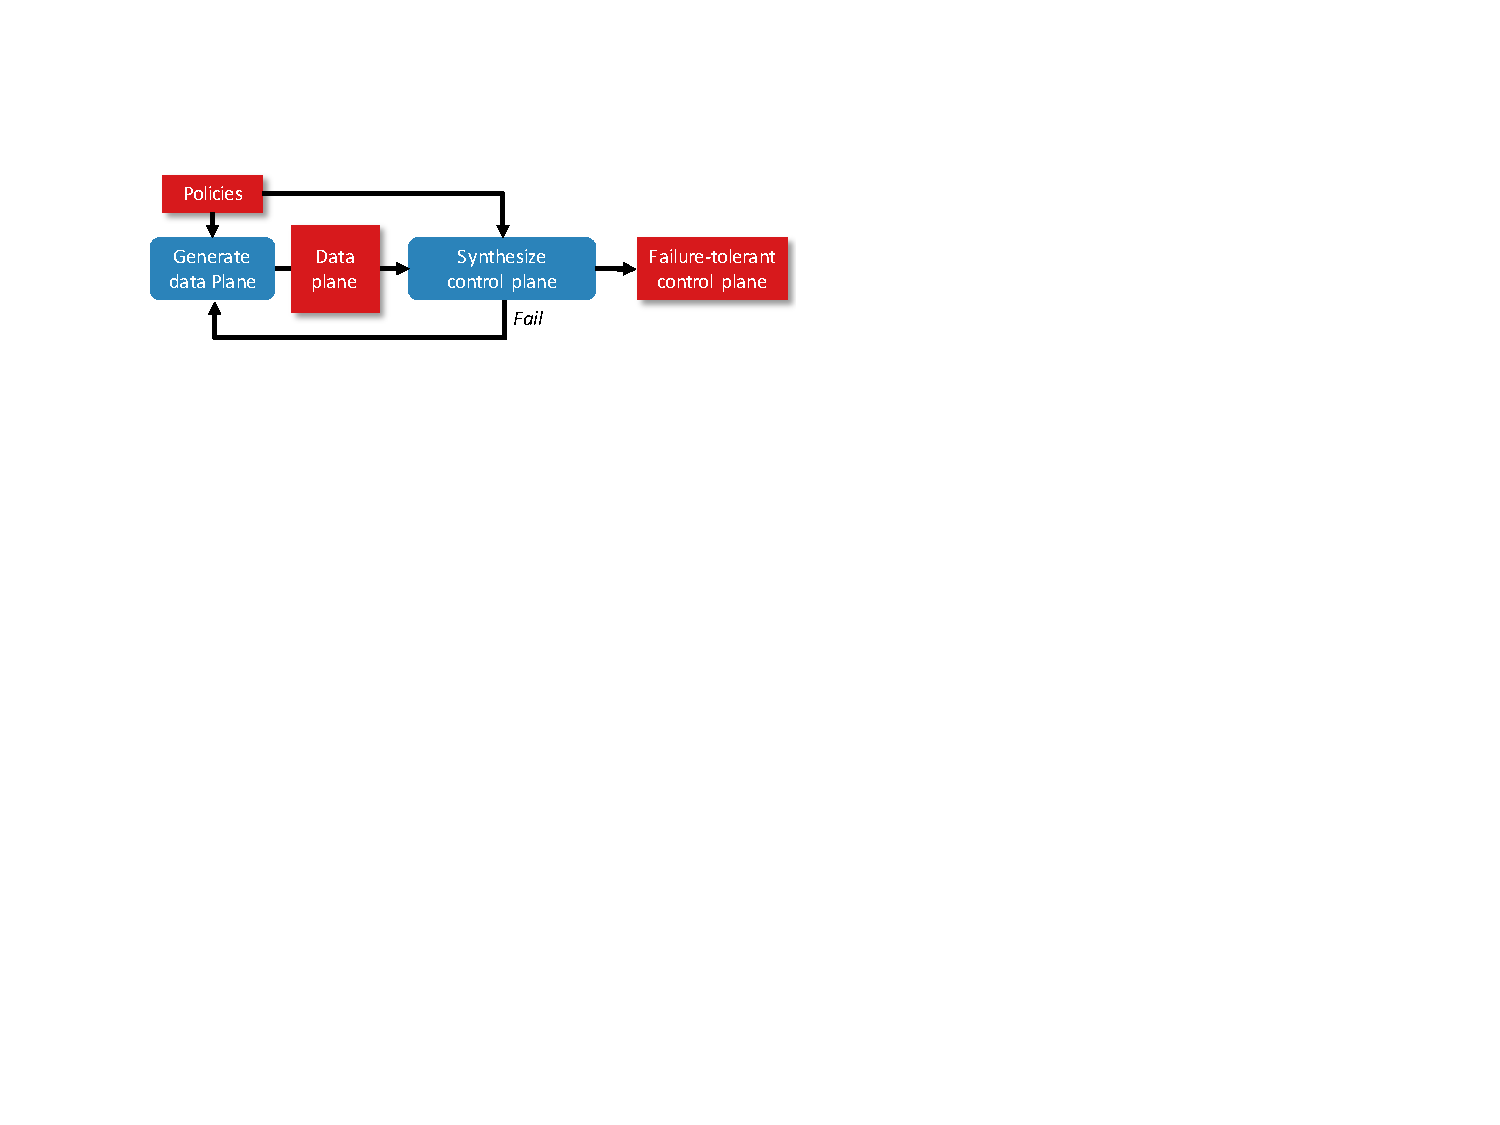
\includegraphics[width=\columnwidth]{figures/architecture.pdf}
%% \compactcaption{Two-phase process for generating a control plane
%%        with failure-tolerance properties}
%% \label{fig:architecture}
%% \end{figure}

\minisection{Configuration Synthesis} To address the aforementioned
challenges, we propose to \emph{automatically synthesize}
policy-compliant configurations.  Given a set of policies describing
path requirements (e.g., reachability, way points, etc.)  and control
plane design requirements (e.g., the number and maximum size of
domains), our goal is to synthesize control plane configurations that
comply with the control-plane requirements and generate paths that
comply with the path requirements. This boils down to investigating two increasingly
hard problems: 1) synthesizing intra- and inter-domain configurations
for routing for a given partition of the network into multiple routing
domains, where each domain uses OSPF shortest-path routing, and
routing across domain is based on BGP local preferences and static
routes (\S~\ref{sec:config-synthesis}); 2) synthesizing configurations
as well as domain assignments i.e., decide how routers are grouped
into different domains which satisfy the input policies
(\S~\ref{sec:synth-dom-ass}).  Since we support complex
policies---e.g., traffic isolation and waypoints---as well as complex
routing techniques---e.g., OSPF and BGP---both configuration synthesis
problems are computationally hard.  We present solutions to these
synthesis problems in the following sections. For the former, we use
constraint solving to generate OSPF weights and domain-specific
techniques to generate BGP preferences. For the latter, we use stochastic
search to explore the space of possible domain assignments.
